\section{Introduction}
\subsection{Overview}
Carcassonne is a tile-based board game for two to five players.  The game board
is a medieval landscape built by the players as the game develops. There is a
initial tile on board, and abound 70 other tiles shuffled face down for the
players to draw from.  Each player takes turn to draw a tile and places it
adjacent to tiles that are already on board. The new tile must be placed in
such a way that extends the regions that is at the edge of the tiles it is
adjacent to.  In particular, roads must connect to roads, fields to fields and
cities to cities.  Besides these three types of features, there is another
feature called `cloister'.  After placing a tile, the player can opt to place a
`follower' on a region of the newly-placed tile. The game ends when all the
tiles are placed.  At that time, each follower on board will be scored for
points according to the regions it is occupying.  Traditionally, the human
players have to view the game board and calculate the scores manually. This is
sometimes time consuming, because there may be many regions and followers on
board.  Furthermore, the score rule is based on the concept of regions, which
makes it nearly impossible to calculate the scores in a simple glimpse.  Even
an experienced player may make mistakes due to the potential possibilities of
connectivity of the regions.  Thus, this motivates us to develop a compute
program that can automatically computes the scores given a final game board
setting.  The program can be written as an cell phone application.  The ideal
scenario will be that after playing a game, one can use a cell phone to take a
photo, and the program reports the scores.  Our program is written in Matlab,
but the methodology can be easily implemented and ported to a cell phone using
required programming language.

\begin{figure}[b]
\centering
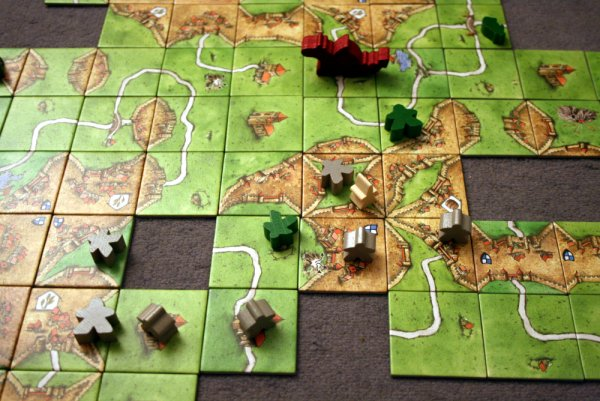
\includegraphics[height=.2\textheight]{board.jpg}
\caption{A part of a game board after several turns (image from
wikipedia).}
\label{fig:board}
\end{figure}

\subsection{Scoring Rules}
Now we introduce the scoring rule after the game finishes.
Note that we deliberately omits the rules when the game is going on,
since we are only focusing on the final game board.
After the game finishes, there will be some incomplete features (regions)
on board. The scoring rules for each feature is as follows:
\begin{itemize}
  \item Road: 1 point per tile.
  \item City: 1 point per tile and 1 point per pennant (a special mark
    that appears in some city features).
  \item Cloister: 1 point itself and 1 point for each surrounding tile.
  \item Field: 3 points for the player who has the most farmers in each
    farm supplying each completed city. This is the most complicated rule,
    since it requires us to explore the field and seek if an adjacent city
    is completed.
\end{itemize}

\subsection{Our Approach}
We first make a few assumptions to the inputs.  One major problem of many
computer vision application is due to occlusion.  In our case, the follower
placed may blocked some of the visible features, which makes it hard for a
computer program to identify the region.  To simply the problem, we require two
images to be taken at the end of game.  In particular, we should first take a
photo for the game board that \emph{contains} the followers, and another one
after removing all of the followers. We further assume that the photos are
taken from a top down view such that there is no perspective distortion of the
tiles, i.e., all tiles are nearly rectangles. Moreover, the game board
must be aligned to the edge of the view plane. Note that these requirements
should not be hard to satisfy. Indeed, we can always compute a perspective
transformation to align the game board. However, we just use assumptions
to focus on the main problem and make our life a bit easier.

The main problem we are facing is to segment the meaningful regions (e.g.,
fields and cities) out from the game board and identify followers to score
them. We have two observations:
\begin{itemize}
  \item Each tile has a regular structure:
   it has four edges, which can be a road, a city or a field segment.
   The center of the tile also contains the following types of features:
   end of a road, cloister, city segment, and field.
 \item Although there are more than 70 pieces of tiles in a standard pack,
   which is the game version we are considering, there are only 
   about 20 types of tiles. Particularly, some tiles will have the same
   structure, except for some decorating elements such as rocks
   that will make the appearance vary.
\end{itemize}
Thus, this motivates us to do such:
pre-compute the region information and visual features of each tile and store
them as templates, match the tiles on game board to find the corresponding
region informations. This is the basic idea of our approach.

Given two input images, one with follower and one without, 
the main flow of the program is as follows:
\begin{itemize}
\item Tile extraction.
In this step, we want to extract each tiles so that 
they can be matched to the template tiles later.
In other words, we want to segment a set of images that
corresponds to separate tiles from one given image.
\item Tile matching.
After extracting the tile images, we can perform image matching.
Our approach is based on SIFT local descriptors and nearest neighbors.
This will be further discussed.
\item Follower detection and region recognition
For each tile image, we also want to know if there is an follower.
If yes, we want to know its color and place such that we can 
identify the region it is occupying and score it for the corresponding player.
\item Connection graph and region map
  After the extraction and matching, we can build a graph
  that contains the connectivity information.
  From this graph, we can apply graph searching to build up the 
  region information.
\item Scoring. Finally, for each follower, we score them according
  to the regions they are occupying using the connection graph and
  region map.
\end{itemize}

In the following sections, we will introduce the technical details
of each step. 
Section~\ref{sec:extract}$\sim$\ref{sec:score} introduce the details
of each step as described as above.
Section~\ref{sec:expr} gives an example of executing our program
on some real world examples.
Finally, a conclusion is drawn in Section~\ref{sec:conclusion}.
